\documentclass{article}

\usepackage{graphicx}
\usepackage{multirow}
\usepackage{color}
\usepackage[colorlinks,
            linkcolor=black,
            anchorcolor=black,
            citecolor=black
            ]{hyperref}
            
\title{DNA De novo Sequence Assembly Review}
\author{Sun Zhao}

\begin{document}
\maketitle
\newpage

\begin{abstract}
The abstract abstract.
\end{abstract}

\section{Before Everything}
I would like to first explain the motivation of this article at the beginning. The theme of this article is about sequence assembly which is a computer aided process for constructing gene sequence. It is actually belonging to the scope of bioinformatics. As a pure computer science undergraduate student, I have started researching in this field since the summer in 2010. After reading lots of papers, discussing with biology researchers from China as well as foreign ones, trying kinds of bioinformatic tools, I approached nothing new but valuable experiences of it. In this article, I will answer the questions of ``what is gene sequencing", ``what is sequence assembly and its challenge", ``how to assembly sequence", ``how to evaluate sequence assembly softwares" and my own contribution to sequence assembly in a computer science researcher's perspective. I'am not going to tell the deep details but giving initiations about what to do and how to do about sequence assembly. Moreover, I will provide valuable references of related papers and materials to help you get a full view of sequence assembly.
\section{What is gene sequencing}
In genetics and biochemistry, sequencing means to determine the primary structure of an unbranched biopolymer. The biopolymer can be DNA, RNA, protein. In this article, I will focus on DNA and RNA sequence analysis excluding protein. DNA sequencing is the process of determining the nucleotide order of a given DNA chain. Concretely, DNA is a chain of four types nucleotide, represented by letter of `A', `G', `C', `T'. DNA sequencing is trying to produce the corresponding string of `A', `G', `C', `T' for a sample DNA chain. However, the most popular biology sequencing method called shot gun, randomly cut the original DNA chain into fragments and a set of `A', `G', `C', `T' strings. Each nucleotide string which is the sequence of a fragment is called a read. To increase the read coverage and read quality, copies of DNA made by PCR amplification with a typical bacteria template are sequenced. Fig. \ref{shot_gun_method} shows the shot gun process, and you may find that reads are sequenced from the two ends of DNA fragments instead of the complete one. The end sequencing phenomena is caused by biology sequencing methods, however, if particular reaction and methods are included, the distance between the two ends can be estimated. In this case, the two end reads are called pair-end reads and the distance is called insert length.\\
\begin{figure}[ht]
  \centering
  % Requires \usepackage{graphicx}
  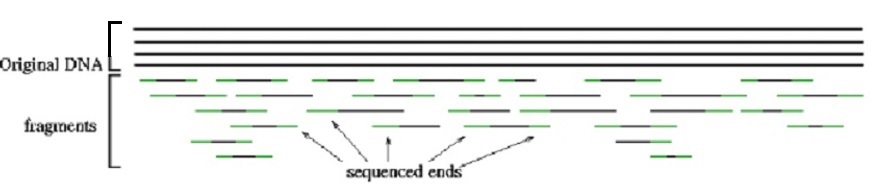
\includegraphics[width=8cm]{Figure1.jpg}\\
  \caption{}\label{shot_gun_method}
\end{figure}
DNA molecules are double-stranded helices, consisting of two long complement strands. According to base paring principle--`A' complements with `T' and `G' complements with `C', the sequence of a strand can be inferred from its opposite one. Particular sequences denoted by 3' and 5' in the DNA strand is used to specify the orientation of the two strand, and for simplicity, if one strand is specified as 3' to 5', then the opposite one is 5' to 3'. Example 1 shows a double strain DNA fragment with pair-end reads(red string). Note that the pair-end reads are positioned on opposite strand and will be sequenced all from 3' to 5'. So the two pair-end reads string should be `AGCTAA' and `GCCAA'.
\begin{center}
  3'$\rightarrow$5'\\
  {\color{red}AGCTAA}TGCTATCTTGGC\\
  TCGATTACGATAG{\color{red}AACCG}\\
  5'$\rightarrow$3'\\
  Example 1\\
\end{center}

\noindent Sequencing methods and platform is developing as time goes. The typical genome analyser of first generation is Sanger\cite{sanger1977nucleotide} producing read lengths of approximately 800bp (typically 500-600bp with non-enriched DNA).Recently, new sequencing methods have emerged \cite{mardis2008impact}. Commercially available technologies include 454 Sequencing \cite{margulies2005genome}, Illumina genome analyser \cite{bentley2006whole} and SOLID sequencing(\href{www.appliedbiosystems.com}{www.appliedbiosystems.com}). Compared to traditional Sanger methods, these technologies function with significantly lower production costs and higher throughput. However, the reads produced by these next-generation sequencing technologies are much shorter than traditional Sanger reads, currently around 400-500 base pairs (bp) for 454, 50bp for Illumina and 35bp for SOLiD. Because of their length, they must be produced in large quantities and at greater coverage depths than earlier sequencing projects.\\
Reads are saved as a file by sequencing chip and the most popular format of read file is FASTA and FASTQ. A sequence in FASTA format begins with a single-line description, followed by lines of sequence data. The description line (def-line) is distinguished from the sequence data by a greater-than (``$>$") symbol at the beginning. It is recommended that all lines of text be shorter than 80 characters in length. An example sequence in FASTA format is shown in Fig. \ref{fasta_format}.A FASTQ file normally uses four lines per sequence. Line 1 begins with a '@' character and is followed by a sequence identifier and an optional description (like a FASTA title line). Line 2 is the raw sequence letters. Line 3 begins with a '+' character and is optionally followed by the same sequence identifier (and any description) again. Line 4 encodes the quality values for the sequence in Line 2, and must contain the same number of symbols as letters in the sequence. A minimal FASTQ file might look like this Fig. \ref{fastq_format}. For more details about the quality line, please refer introduction on \href{http://en.wikipedia.org/wiki/FASTQ_format}{FASTQ Format}.\\
The last thing to mention is RNA sequencing. As RNA is generated by transcription from DNA, the information is already present in the cell's DNA. The usual method to sequence RNA is first to reverse transcribe the sample to generate cDNA fragments. Then the cDNA are sequenced using DNA sequencing methods.\\
In a word, the next generation sequencing platform generates a FASTA/FASTQ format file consisting string of description, read and quality(only exists in FASTQ file) for DNA/RNA samples.
\begin{figure}[ht]
  \centering
  % Requires \usepackage{graphicx}
  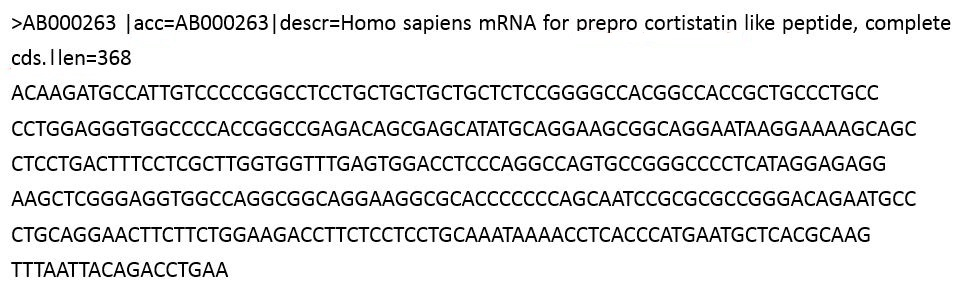
\includegraphics[width=10cm]{Figure2.jpg}\\
  \caption{}\label{fasta_format}
\end{figure}
\begin{figure}[ht]
  \centering
  % Requires \usepackage{graphicx}
  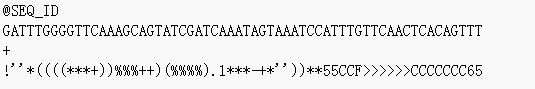
\includegraphics[width=10cm]{Figure3.jpg}\\
  \caption{}\label{fastq_format}
\end{figure}
\section{What is sequence assembly}
What the sequencing stage produces is a collection of DNA fragments's nucleotide sequence, whereas, what we need is the nucleotide sequence of the original one. Sequence assembly tries to align and merge the DNA fragments in order to reconstruct the original sequence. The intuition is to take advantage of overlap information between reads to tie them up and piece into a longer DNA sequence. Challenges listed blow makes sequence assembly a very complicated task.\\
\begin{itemize}
 \item One cell contains multiple chromosomes as well as DNA chains which are sequenced together. DNA fragments from different DNA chain may overlap.
 \item DNA is a double-stranded structure, one strand may overlap with its opposite one.
 \item Sheared fragments along the genome cannot be modeled as a perfect Poisson process so that there may be some region not covered by reads. 
 \item DNA sequence may contains repeat regions, and these regions may be incorrectly merged by overlap.
 \item Sequencing errors causes nucleotide deleting, replacing or inserting inside reads.
 \item Second generation sequencing platform produces much shorter reads so that the overlap possibility is exponentially increased. 
\end{itemize}
Among those above challenges, the repeat problem is the most challenge thing for short read assembly. A simple example is shown in Fig. \ref{repeat_example}A, where the assembler incorrectly collapses the two copies of repeat A leading to the creation of two contigs instead of one Fig. \ref{repeat_example}B.\\
\begin{figure}[ht]
  \centering
  % Requires \usepackage{graphicx}
  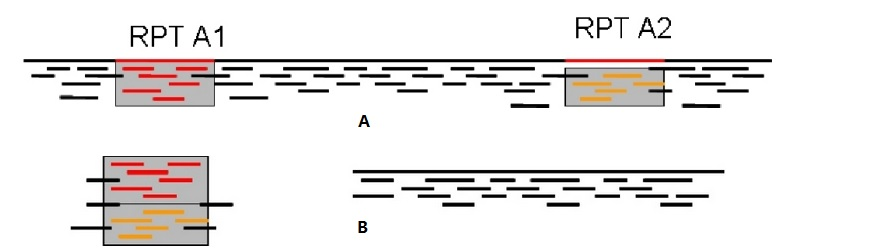
\includegraphics[width=10cm]{Figure4.jpg}\\
  \caption{}\label{repeat_example}
\end{figure}
\noindent The basic strategies for assembling sequences are categorized by two groups. One is reference based assembly, and the other one is de novo assembly. Reference based methods using a mapping tool to align reads against an existing reference sequence and build a sequence that is similar but not necessarily identical to the reference. The de novo assembly strategy does not use a reference sequence and is much useful for species whose reference sequence are unknown. This article only covers the de novo assembly and will illustrate the details in the subsequent sections.\\
Ideally, an assembly program should produce one contig for every chromosome of the genome being sequenced. However, because of challenge3 and challenge4, the output of the assembler is interrupted into a set of contigs. In summary, Inputting a FASTA/FASTQ read file, the assembler outputs a set of contigs.
\section{How to assembly sequence}
Overlap-consensus-layout \cite{myers1995toward} is the traditional approach for first generation sequence. It denotes each read as a separate node, where two reads presenting a clean overlap are connected by a bidirected edge. Although overlap-consensus-layout approach is both intuitive and robust, especially in the case of long reads, it is very costly for pair-wise overlap computing when assembling high quantity short reads produced by second generation sequencing platform like SOLID and Illumina. Only one microread assembler, EDENA \cite{hernandez2008novo} was developed using this approach. Later, Idury and Waterman \cite{idury1995new} introduced the use of a sequence graph to represent an assembly, and this idea has been developed into the most popular framework for short read assembly--De Bruijn graph. Sequence De Bruijn graph is constructed from a set of kmers(k is a parameter) as nodes, and two kmers are connected if one kmer's last k-1 nucleotides is identical to the first k-1 nucleotides. kmers are produced by moving a fixed length(k) sliding window on the original read. The sequence de bruijn graph has following properties:
\begin{itemize}
 \item Read with length of n generates n-k+1 kmers.
 \item Read is mapping to a unique path in the de bruijn graph.
 \item One node has at most 4 successors and 4 predecessors by adding `A', `G', `C', `T' at the first or last of the k-1 nucleotides.
\end{itemize}
\renewcommand\refname{Reference}
\bibliographystyle{plain}
\bibliography{Thesis}
\end{document}
